\chapter{Graph Exploration and Structural Insights}
\label{chap:graph_exploration}

\section{Why Explore the Graph Before Prediction?}

It is tempting to treat the graph built in Chapter~\ref{chap:kg} as a
black box that is fed into a GNN and evaluated by a single F1 number.
That view is wrong for two reasons.

First, \emph{the graph is the dataset}. In a flat-text pipeline the
dataset is a set of labelled documents; here the dataset is a typed,
relational object with cross-domain structure, and any claim a later
chapter makes about the model's behaviour presupposes a concrete
understanding of that structure. Whether the model's accuracy is
driven by genuine cross-case reasoning or by a few dominant hub
statutes, whether the five legal domains are actually five or mostly
one, whether the per-case subgraph has the connectivity a
message-passing layer needs -- none of these questions can be answered
by looking at prediction results alone.

Second, \emph{leakage-safety claims are structural claims}. The
leakage prevention strategy in
Section~\ref{sec:leakage_prevention} is only as convincing as the
structural evidence that the remaining graph is still dense enough to
support learning. If removing RPC annotations, decision fields, and
identity-proxy shortcuts left behind a near-disconnected graph, the
downstream accuracy would be either implausibly high (still leaking)
or implausibly low (now uninformative). The exploration stage is
where we verify that neither is the case.

This chapter therefore treats the graph as an object of study in its
own right. Section~\ref{sec:graph_stats} summarises the overall
structure; Section~\ref{sec:perdomain} breaks it down per legal
domain; Section~\ref{sec:key_insights} distils the conclusions that
feed forward into Chapter~\ref{chap:results}.

\section{Graph Statistics and Structural Analysis}
\label{sec:graph_stats}

\subsection{Overall Graph Statistics}

The final reasoning-focused graph, assembled across all five legal
domain buckets, contains \textbf{880{,}176 nodes} and
\textbf{1{,}977{,}295 edges}. The average node degree is
\textbf{4.49}; the maximum degree is \textbf{29{,}602}, attained by
the \textsc{IPC} statute node.

At the per-bucket level (before cross-bucket sharing is expanded into
the unified view the GNN trains on), the five buckets have broadly
comparable case counts but markedly different internal densities:

\begin{table}[H]
  \centering
  \small
  \begin{tabular}{lrrr}
    \toprule
    Bucket & Cases (files) & Nodes & Edges \\
    \midrule
    Family \& Matrimonial & 15{,}307 & 97{,}150 & 3{,}660{,}068 \\
    Financial Fraud & 14{,}616 & 113{,}240 & 7{,}869{,}952 \\
    Land \& Property & 14{,}052 & 126{,}962 & 9{,}210{,}612 \\
    Motor Accidents & 15{,}237 & 125{,}234 & 7{,}165{,}461 \\
    Sexual Offences & 14{,}597 & 106{,}662 & 7{,}123{,}225 \\
    \midrule
    \textbf{Cross-bucket unified} & \textbf{73{,}809} & \textbf{485{,}540}
      & \textbf{27{,}243{,}141} \\
    \bottomrule
  \end{tabular}
  \caption{Per-bucket and cross-bucket graph statistics. The
  cross-bucket graph is denser than the sum of the per-bucket graphs
  because shared \textsc{Statute}, \textsc{Provision}, and
  \textsc{Precedent} nodes acquire edges from every bucket that cites
  them.}
  \label{tab:graph_stats}
\end{table}

Family-matrimonial is the sparsest bucket by edges-per-case
(\(\approx 239\)), and land-property is the densest (\(\approx 655\));
the difference is driven mostly by the number of distinct provisions
and precedents cited per case in each domain.

\subsection{Node Type Distribution}

The node-type breakdown of the unified graph is strongly skewed
towards \textbf{parties and precedents}:

\begin{table}[H]
  \centering
  \small
  \begin{tabular}{lrr}
    \toprule
    Node type & Count & Share \\
    \midrule
    \textsc{Case}        &  72{,}735 &  8.3\% \\
    \textsc{Precedent}   & 255{,}148 & 29.0\% \\
    \textsc{Respondent}  & 192{,}147 & 21.8\% \\
    \textsc{Petitioner}  & 171{,}084 & 19.4\% \\
    \textsc{Lawyer}      &  73{,}645 &  8.4\% \\
    \textsc{Provision}   &  43{,}504 &  4.9\% \\
    \textsc{Court}       &  38{,}799 &  4.4\% \\
    \textsc{Statute}     &  21{,}754 &  2.5\% \\
    \textsc{Judge}       &  11{,}360 &  1.3\% \\
    \bottomrule
  \end{tabular}
  \caption{Distribution of the 880{,}176 nodes by type in the unified
  reasoning-focused graph.}
  \label{tab:node_type_dist}
\end{table}

\begin{figure}[H]
  \centering
  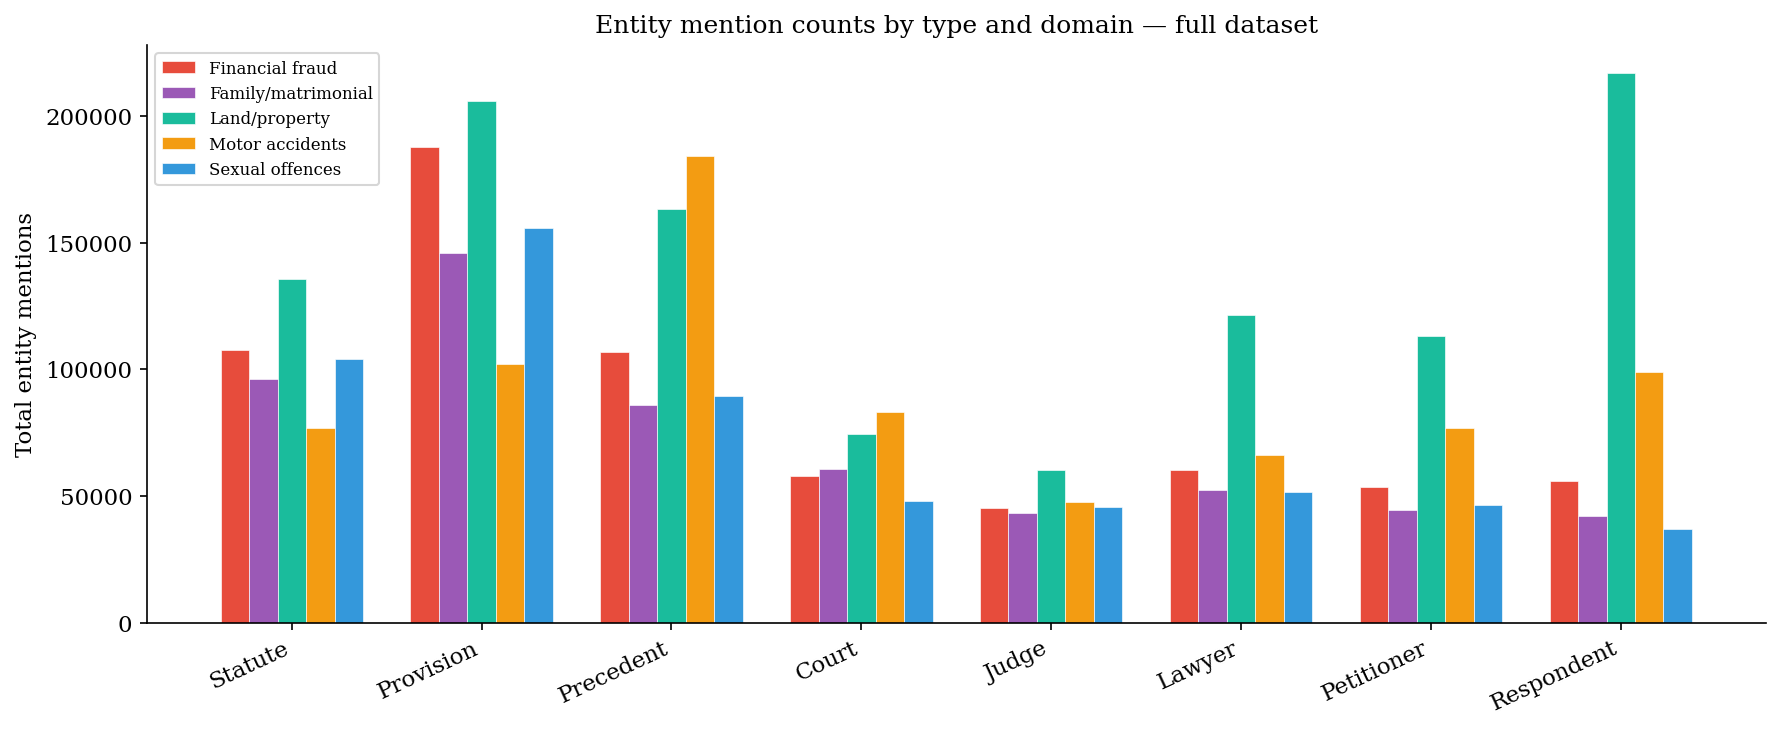
\includegraphics[width=0.92\textwidth]{figures/entity_type_totals_full.png}
  \caption{Entity type totals across the corpus.}
  \label{fig:entity_type_totals}
\end{figure}

Two observations follow. First, precedents outnumber every other
non-party type by an order of magnitude -- citation is by far the
dominant legal artefact in the graph, which is why precedent sharing
is a load-bearing edge type. Second, parties (\textsc{Petitioner} +
\textsc{Respondent}) account for more than $40\%$ of nodes; because
they are held \emph{local} to each case rather than shared, they
contribute many nodes but no cross-case edges. The statute side of
the graph is small in node count but, as the next subsection shows,
carries disproportionate structural weight.

\subsection{Degree Distribution and Hub Entities}

The graph is strongly hub-dominated. The top-12 nodes by degree are
all statutes, provisions, or courts -- exactly the node types the
schema shares across cases:

\begin{table}[H]
  \centering
  \small
  \begin{tabular}{llrr}
    \toprule
    Node & Type & Degree & Buckets bridged \\
    \midrule
    IPC                                   & Statute   & 29{,}602 & 5 \\
    CR.P.C.                               & Statute   & 18{,}704 & 5 \\
    Supreme Court                         & Court     & 17{,}294 & 5 \\
    Apex Court                            & Court     & 14{,}242 & 5 \\
    Indian Penal Code                     & Statute   & 12{,}009 & 5 \\
    High Court of Judicature at Allahabad & Court     &  8{,}833 & 5 \\
    Section 482                           & Provision &  8{,}732 & 5 \\
    Section 506                           & Provision &  8{,}258 & 5 \\
    I.P.C.                                & Statute   &  7{,}051 & 5 \\
    Section 420                           & Provision &  6{,}285 & 5 \\
    Section 323                           & Provision &  6{,}002 & 5 \\
    Constitution of India                 & Statute   &  5{,}950 & 5 \\
    \bottomrule
  \end{tabular}
  \caption{Top hub entities by degree, with the number of buckets they
  bridge. Every one of the top 12 hubs appears in all five legal
  domains.}
  \label{tab:top_hubs}
\end{table}

The PageRank ranking tells the same story from a different angle:
IPC ($\text{PR}=0.0114$), Supreme Court ($0.0082$), CR.P.C.\
($0.0069$), and Apex Court ($0.0067$) dominate the top of the
distribution. That every one of the top hubs bridges all five buckets
is not an accident of the numbers -- these are the statutes and
courts every Indian criminal and civil proceeding touches -- but it
has a concrete modelling consequence: these hubs are where cross-case
message passing actually happens.

The corollary is that the graph has \emph{many} near-isolated nodes
too. Most precedents appear in a single case; most parties appear in
one matter; most judges hear a bounded docket. This two-regime
structure -- a small set of super-hubs plus a long tail of
single-case leaves -- is what the ``connectivity score''
(Section~\ref{sec:connectivity}) is designed to quantify.

\subsection{Cross-Domain Bridge Analysis}

The buckets are not isolated. Table~\ref{tab:top_hubs} already shows
that the top hubs are bridges by construction; the full bridge
analysis confirms that the connective tissue between domains is
dominated by the general criminal-procedure and penal-code statutes,
with domain-specific bridges layered on top:

\begin{itemize}
  \item \textsc{IPC}, \textsc{CR.P.C.}, \textsc{Indian Penal Code},
    \textsc{Constitution of India}, and \textsc{Supreme Court} /
    \textsc{Apex Court} appear in all five buckets and together account
    for the majority of cross-bucket edges.
  \item Domain-specific statutes bridge fewer buckets but at higher
    within-bucket intensity: \textsc{POCSO Act} appears in four
    buckets but is heavily concentrated in sexual-offences;
    \textsc{Motor Vehicles Act, 1988} appears in all five but is
    concentrated in motor-accidents; \textsc{Land Acquisition Act,
    1894} is concentrated in land-property.
  \item Provisions like Section~482, 506, 420, and 323 are multi-bucket
    because they sit in the CrPC and IPC, which are themselves
    multi-domain.
\end{itemize}

\begin{figure}[H]
  \centering
  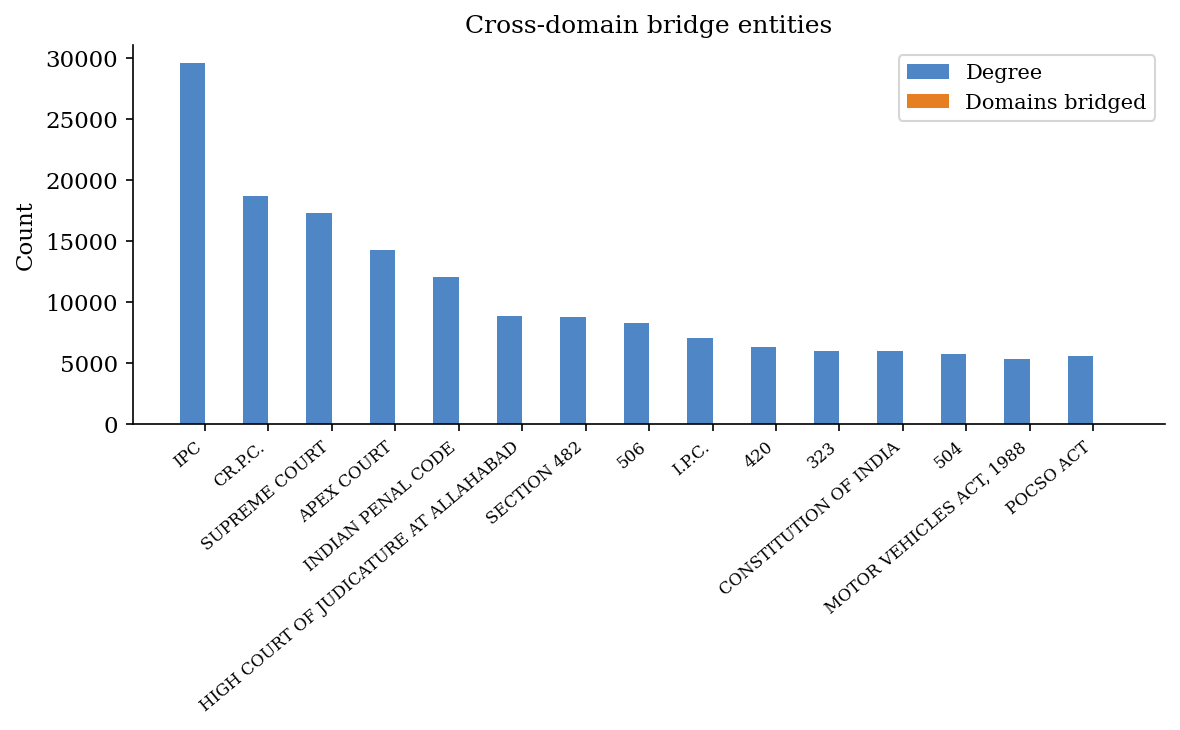
\includegraphics[width=0.92\textwidth]{figures/cross_bucket_bridges.png}
  \caption{Cross-bucket bridges: entities that connect more than one
  legal domain, ranked by the number of buckets they appear in.}
  \label{fig:cross_bucket_bridges}
\end{figure}

\begin{figure}[H]
  \centering
  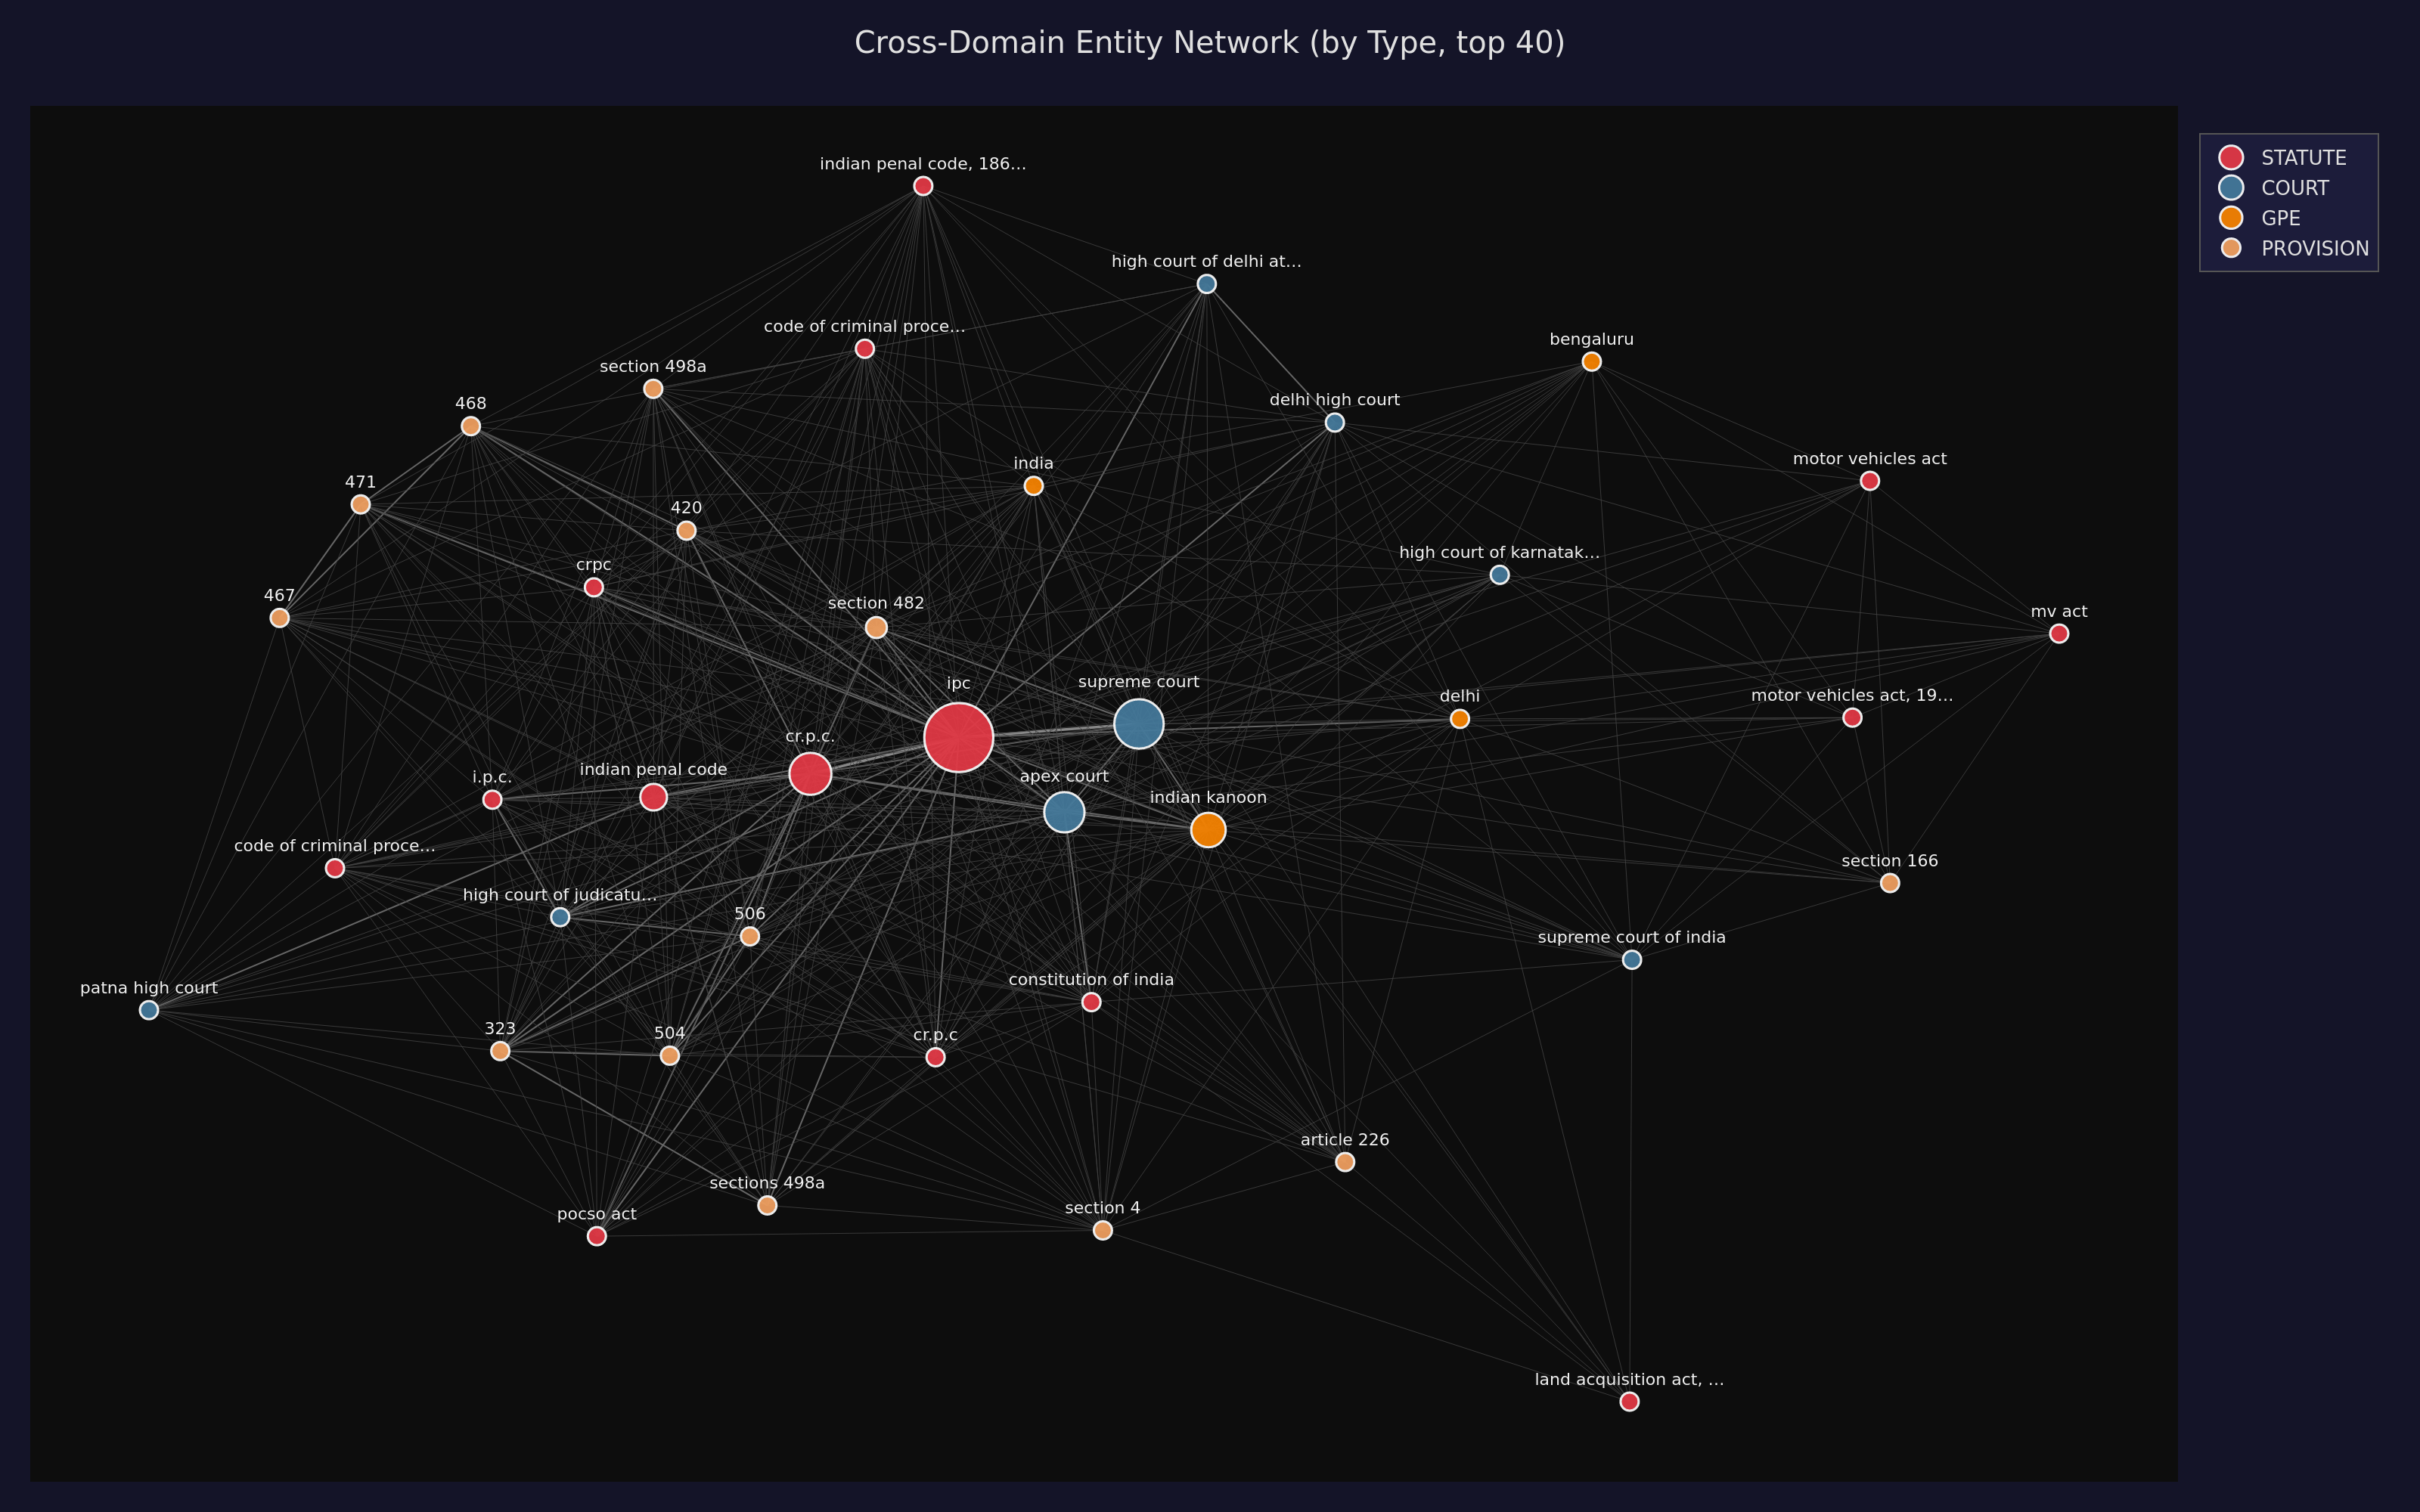
\includegraphics[width=0.95\textwidth]{figures/cross_bucket_network_by_type_readable.png}
  \caption{{\color{blue}Cross-domain entity network for the highest-PageRank
  shared entities, coloured by node type. Unlike the bridge-count bar
  chart, this view shows the \emph{shape} of the shared legal spine:
  which entities form the dense centre, and which remain peripheral
  even when they appear across multiple domains.}}
  \label{fig:cross_bucket_network_topology}
\end{figure}

{\color{blue}Figure~\ref{fig:cross_bucket_network_topology} adds a
topological point that the aggregate bridge counts alone do not make
visible. The cross-domain backbone is narrow and authority-driven:
\textsc{IPC}, \textsc{Cr.P.C.}, \textsc{Supreme Court}, and
\textsc{Apex Court} occupy the centre, while bucket-specific statutes
such as the \textsc{Motor Vehicles Act}, \textsc{POCSO Act}, and
\textsc{Land Acquisition Act} attach as secondary clusters rather than
co-equal hubs. A further visual detail is that \textsc{GPE} nodes
(\emph{Indian Kanoon}, Delhi, Bengaluru) sit mostly on the outside of
the network. They co-occur often enough to be visible, but they do not
organise the graph the way statutes, provisions, and courts do. This
sharpens the interpretation of cross-domain transfer: message passing
is not occurring through a uniformly shared legal space, but through a
small common authority backbone that then branches into
bucket-specific statutory neighbourhoods.\par}

\subsection{Entity Sharing Heatmap Across Domains}

The entity-sharing heatmap
(Figure~\ref{fig:entity_sharing_heatmap}) visualises, for each
pair of buckets, the number of shared canonical entities. Three
patterns are visible:

\begin{enumerate}
  \item a strong sharing between \emph{Family \& Matrimonial},
    \emph{Financial Fraud}, and \emph{Sexual Offences}, all of which
    are IPC/CrPC-driven;
  \item moderate sharing between those three and \emph{Motor
    Accidents}, mediated by the procedural statutes and by the
    Supreme Court / High Court nodes;
  \item comparatively weaker sharing with \emph{Land \& Property},
    which has its own statutory backbone (Land Acquisition Act,
    Constitution).
\end{enumerate}

\begin{figure}[H]
  \centering
  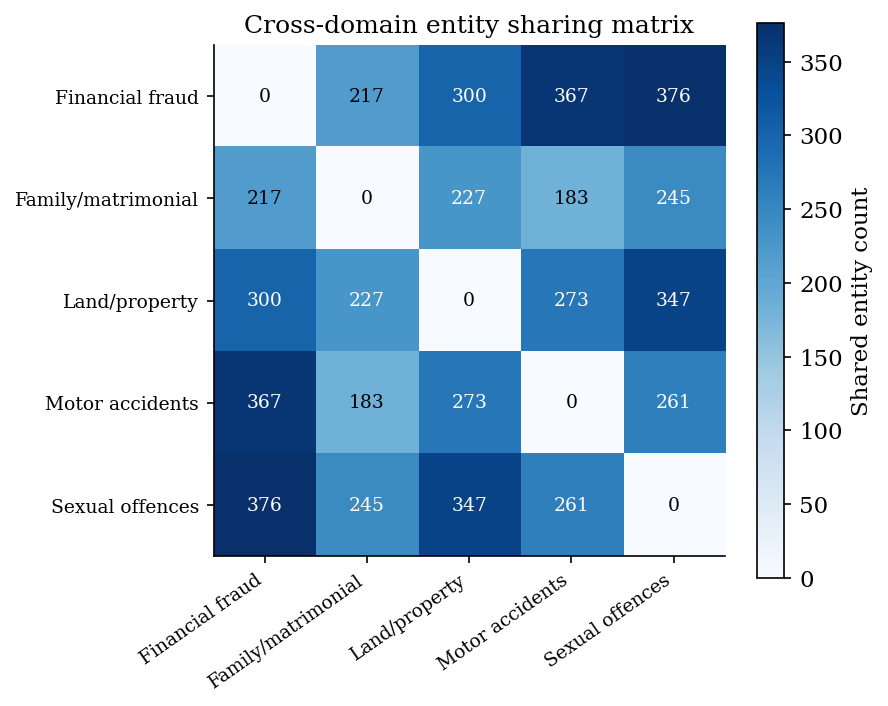
\includegraphics[width=0.9\textwidth]{figures/entity_sharing_heatmap.png}
  \caption{Entity sharing heatmap across the five legal domains.}
  \label{fig:entity_sharing_heatmap}
\end{figure}

This pattern is exactly what a cross-domain transfer claim needs: the
domains are related enough that a shared representation should carry
useful signal, but different enough that a single-domain classifier
should not dominate a cross-domain one unless that shared signal is
actually being used.

\subsection{Connectivity Score Distribution}
\label{sec:connectivity}

A \textbf{connectivity score} is assigned to each case as a
bucket-normalised measure of how well that case is wired into the
rest of the graph through its shared-entity neighbours (statutes,
provisions, precedents). High-connectivity cases cite hub statutes
and widely-cited precedents; low-connectivity cases sit on rare or
single-case entities.

\begin{figure}[H]
  \centering
  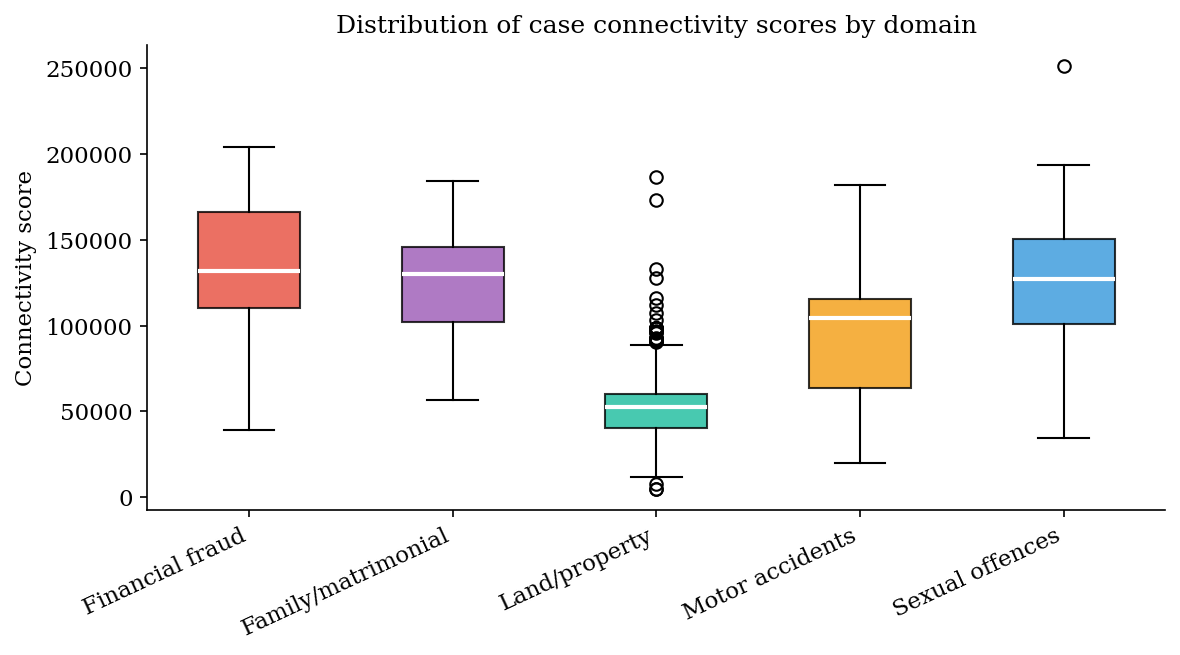
\includegraphics[width=0.9\textwidth]{figures/connectivity_score_distributions.png}
  \caption{Connectivity score distribution per bucket.}
  \label{fig:connectivity}
\end{figure}

The score is used by the Graph Visualiser
(\texttt{GRAPH\_VISUALISER/}) to rank cases when sampling Hub-Network
and Case-Connection views, and is a useful diagnostic for message
passing: a GNN layer's information gain on a low-connectivity case is
structurally bounded, and the ablation pattern in
Chapter~\ref{chap:results} consistent with this expectation.

\section{Per-Domain Corpus Analysis}
\label{sec:perdomain}

The structural view above aggregates across buckets; the per-domain
view is where the legal character of each bucket shows up.

\subsection{Case Length and Sentence Distributions}

Case length varies substantially across buckets. Motor-accidents
judgments are typically short and tribunal-style; land-property
matters are long and document-heavy (deeds, surveys, and possession
history); family-matrimonial sits in the middle, dominated by
petition-style fact sections. Sentence-count distributions follow the
same ordering and are the primary driver of the hierarchical-chunking
configuration in Section~\ref{sec:text_features}: long-tail
\textsc{Facts} and \textsc{Arguments} sections in land-property and
financial-fraud buckets exceed the \texttt{bge-m3} context window and
are mean-pooled across overlapping chunks.

\subsection{Entity Richness Per Domain}

Entity richness -- unique canonicalised entities per case -- is
highest in land-property and financial-fraud, which carry many
distinct parties, precedents, and provisions per matter, and is
lowest in motor-accidents, which repeatedly cites the same small set
of provisions (Section~166, Motor Vehicles Act). The PageRank ranking
within each bucket makes this concrete:

\begin{itemize}
  \item \textbf{Family \& Matrimonial}: IPC, CrPC, Sections~498A,
    482, 498A.
  \item \textbf{Financial Fraud}: IPC, CrPC, Sections~420, 468, 471.
  \item \textbf{Land \& Property}: Supreme Court, Land Acquisition
    Act~1894, \emph{Indian Kanoon} (a source GPE), Constitution of
    India.
  \item \textbf{Motor Accidents}: Supreme Court, Motor Vehicles Act
    1988, Apex Court, Section~166, Motor Vehicles Act.
  \item \textbf{Sexual Offences}: IPC, CrPC, POCSO Act, Indian Penal
    Code, Section~506.
\end{itemize}

The top-5 per bucket is a near-perfect fingerprint of the underlying
legal domain, which is a reassuring sanity check: the canonicalisation
and the NER are recovering legally meaningful primary citations, not
surface noise.

\begin{figure}[H]
  \centering
  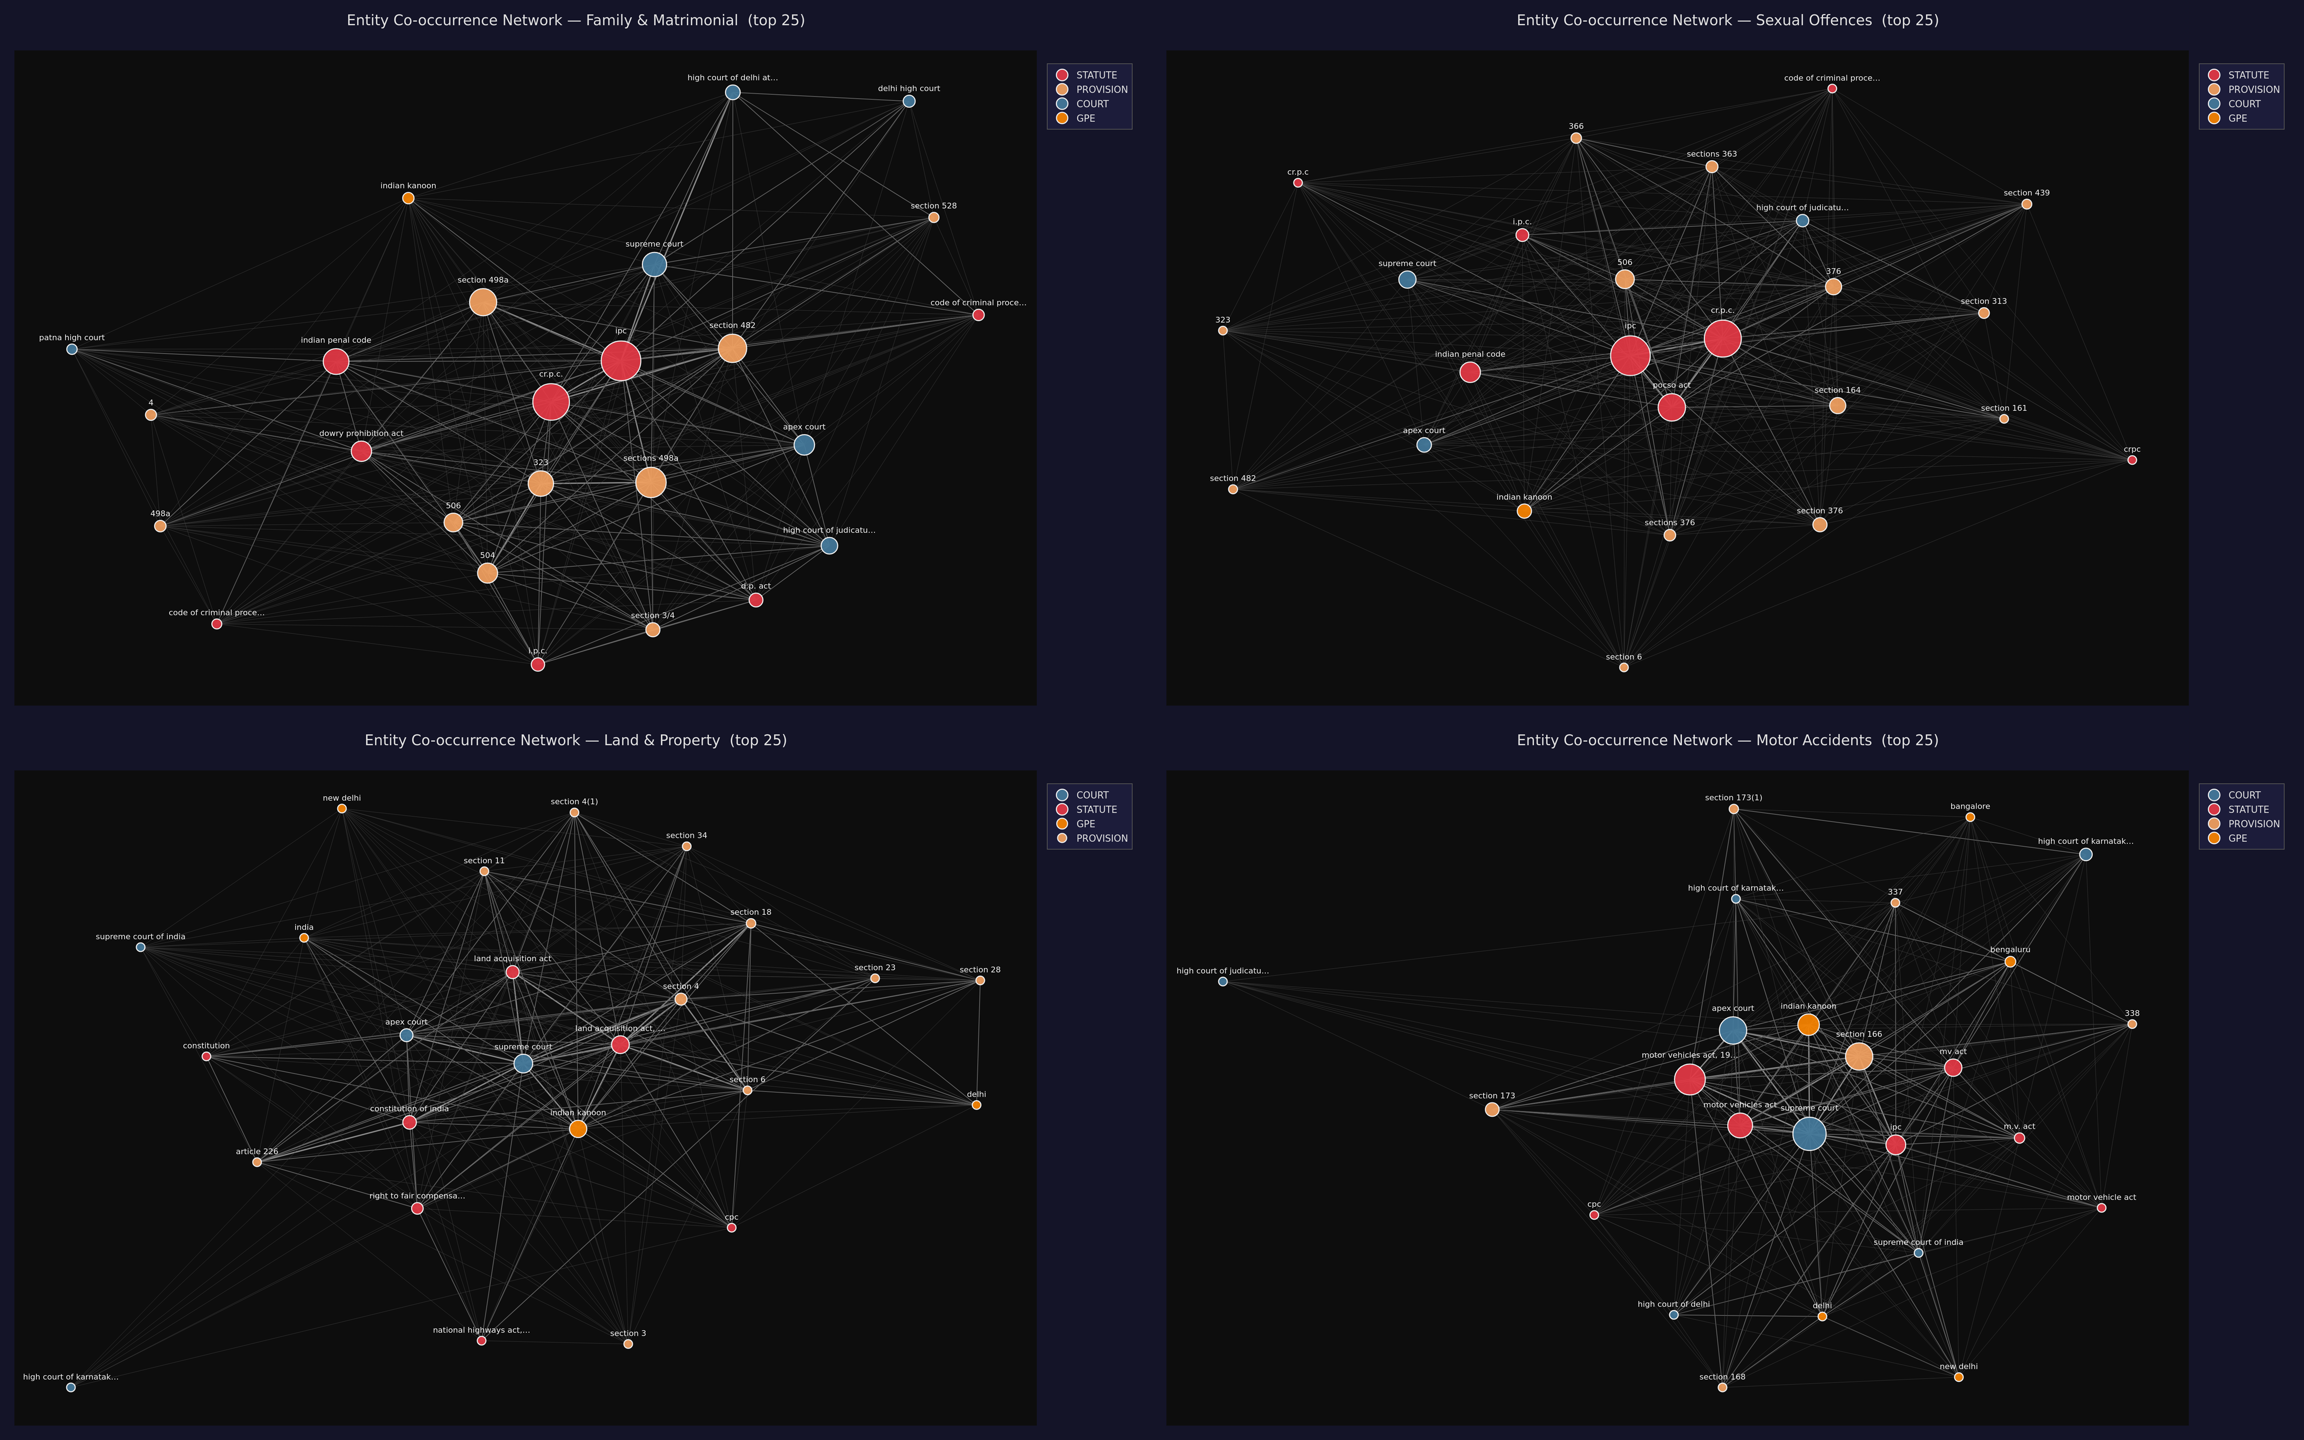
\includegraphics[width=\textwidth]{figures/within_bucket_network_fingerprints.png}
  \caption{{\color{blue}Representative within-bucket entity
  co-occurrence networks for four legal domains, each restricted to the
  top-25 PageRank entities in that bucket. The figure is intended as a
  structural fingerprint view: not just which entities are important,
  but how each bucket's important entities organise into a distinct
  local backbone.}}
  \label{fig:within_bucket_network_fingerprints}
\end{figure}

{\color{blue}Figure~\ref{fig:within_bucket_network_fingerprints}
shows that the domains differ not only in their top entities but in
their \emph{network geometry}. Family \& matrimonial and sexual
offences both remain visibly \textsc{IPC}/\textsc{CrPC}-centred, yet
they split into different provision clusters almost immediately:
Section~498A / 482 and dowry-law citations in the former, versus
\textsc{POCSO} / Section~376 / 363 clusters in the latter.
Land-property is more spatially spread, with several semi-central
statutory and constitutional nodes rather than one overwhelmingly
dominant criminal-procedure core; this is consistent with its higher
entity richness and document-heavy reasoning style. Motor-accidents,
by contrast, exhibits the tightest and most repetitive local backbone
around the \textsc{Motor Vehicles Act} and Section~166, suggesting
that many cases enter the graph through a comparatively narrow set of
recurring authorities. Financial-fraud is omitted here for space, but
its readable network shows the same kind of provision-centred motif
around Sections~420, 468, and 471. Together these bucket-level
snapshots make the earlier ``domain fingerprint'' claim visual rather
than purely tabular.\par}

\subsection{Rhetorical Role Composition Per Domain}

The rhetorical-role composition of each bucket -- once RPC/RLC are
removed by the leakage filter -- is dominated by \textsc{Facts} and
\textsc{Arguments}, with a stable \textsc{Preamble} share across
domains. The relative size of the \textsc{Arguments} block tracks
case length: it is largest in land-property and financial-fraud and
smallest in motor-accidents.

\begin{figure}[H]
  \centering
  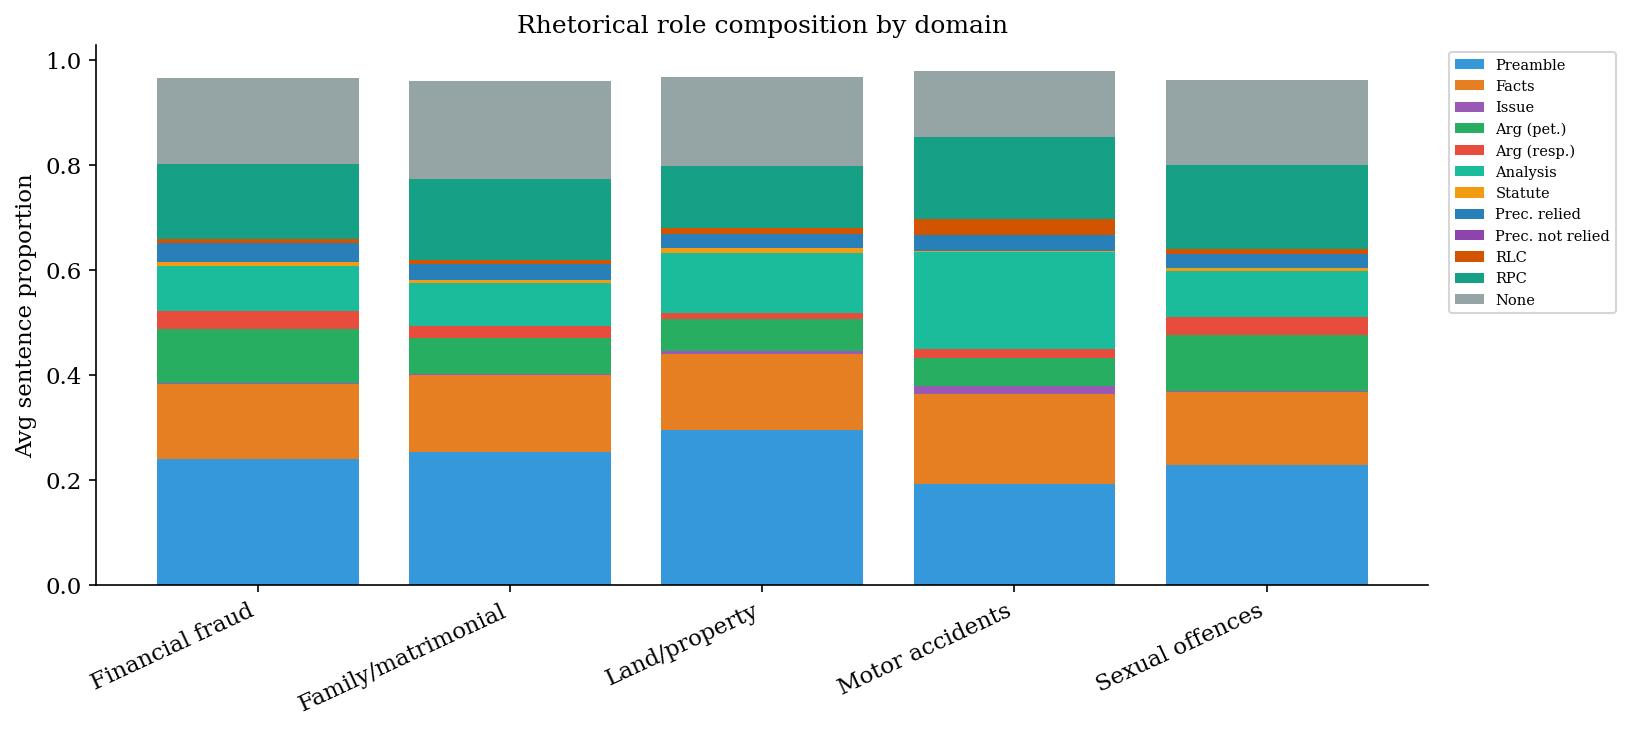
\includegraphics[width=0.95\textwidth]{figures/rhetorical_role_breakdown_full.png}
  \caption{Rhetorical role breakdown per bucket after
  leakage-safe filtering. \textsc{RPC} and \textsc{RLC} annotations
  are intentionally absent.}
  \label{fig:rr_breakdown}
\end{figure}

\subsection{Outcome Distribution Per Domain}

The outcome label distribution (Figure~\ref{fig:outcome_distribution})
is moderately imbalanced and bucket-dependent. Motor-accidents is the
most \textsc{win}-skewed, consistent with compensation claims being
allowed more often than rejected at the appellate stage;
financial-fraud and sexual-offences are closer to balanced. The
cross-bucket pooled distribution is roughly $\sim\!60\%$ \textsc{win}
to $\sim\!40\%$ \textsc{loss}, which is why
Chapter~\ref{chap:results} reports macro-F1 alongside accuracy and
ROC-AUC.

\section{Key Structural Insights}
\label{sec:key_insights}

Five insights carry forward into the prediction chapter:

\begin{enumerate}
  \item \textbf{The graph is hub-dominated.} A small number of
    cross-bucket statutes and courts (IPC, CrPC, Supreme Court) are
    the spine of the graph; most other entities are long-tail leaves.
    Any claim the model makes about ``cross-case reasoning'' must be
    interpretable against this topology.
  \item \textbf{Cross-domain sharing is real but uneven.} The four
    IPC/CrPC-driven buckets share heavily with each other; land-property
    partially detaches via its own statutory backbone. A cross-domain
    model should outperform a naive concatenation only if it can
    actually exploit the shared spine.
  \item \textbf{Identity-proxy leakage is structural.} Judges,
    specific lawyers, and specific courts have bridge and betweenness
    scores high enough to make \emph{sharing} them across cases
    unsafe; the decision to hold them local is vindicated by the
    bridge analysis.
  \item \textbf{Connectivity score predicts modelling difficulty.}
    Low-connectivity cases have, by construction, fewer shared-entity
    neighbours to aggregate from; the per-domain accuracy pattern in
    Chapter~\ref{chap:results} is consistent with connectivity being a
    first-order driver of case-level difficulty.
  \item \textbf{The per-domain fingerprints are legally coherent.}
    Each bucket's top-PageRank entities are exactly what a lawyer
    would expect; this is the single strongest evidence that the
    pipeline's NER, canonicalisation, and rhetorical-role filtering
    together produce a legally faithful, not merely statistically
    clean, corpus.
\end{enumerate}
